\documentclass[10pt,twocolumn]{article}
\usepackage[letterpaper,margin=0.72in,columnsep=0.24in]{geometry}
\usepackage[T1]{fontenc}
\usepackage[utf8]{inputenc}
\usepackage{times}
\usepackage{microtype}
\usepackage{booktabs}
\usepackage{graphicx}
\usepackage{stfloats}
\usepackage[font=small,labelfont=bf,skip=3pt]{caption}
\usepackage[round]{natbib}
\setlength{\bibsep}{0pt}
\usepackage[most]{tcolorbox}
\usepackage[hidelinks]{hyperref}
\usepackage{titlesec}
\titlespacing*{\section}{0pt}{4pt}{1pt}
\titleformat{\section}{\normalsize\bfseries}{\thesection}{0.5em}{}
\setlength{\parskip}{1pt}
\setlength{\parindent}{0pt}
\raggedbottom
\setlength{\textfloatsep}{6pt}
\setlength{\dbltextfloatsep}{6pt}
\newtcolorbox{hypbox}{breakable,colback=gray!8,colframe=gray!60,boxrule=0.4pt,arc=1pt,left=3pt,right=3pt,top=2pt,bottom=2pt}
\newcommand{\XX}[1]{\textcolor{red}{#1}}

\title{\vspace{-0.62in}\large\textbf{Leaving for Europe, or Leaving Science?}\\[2pt]\normalsize Reading Parental Leave Policies at Scale to Explain Who Stays in US Academia}
\author{\normalsize Antoni Czolgowski \quad CSCI 7000 NLP for Cultural Analytics, Proposal 3, 27 October 2026}
\date{\vspace{-0.32in}}

\begin{document}
\maketitle

\section{Motivation and research questions}
Take two women hired as assistant professors in the same year, one at the University of Kentucky and one at the University of Nottingham, two universities of about the same size and mix of fields. Both have their first child. In Nottingham the policy gives her 26 weeks off at full pay. In Kentucky she is paid while she recovers, ``usually 6--8 weeks'', under the faculty rules for temporary disability, and a colleague whose partner gives birth finds no paid leave in those rules at all. At CU Boulder either parent gets 18 weeks at full pay. In the US each university writes these rules, in most of Europe the state does. I read these documents as culture written down: besides the weeks, they say whom the institution imagines as the parent, a mother who has to recover, any parent, or a ``primary caregiver'' who has to declare it. The wording has effects. When top economics departments made tenure-clock extensions gender-neutral, men's tenure rates went up and women's went down \citep{antecol2018}.

I want to know if these rules change who stays in science. Parenthood explains most of the gender gap in faculty productivity, and women, far more than men, say the leave policy mattered when they chose their job \citep{morgan2021}. But a survey of current faculty only hears from those who stayed. In a census of 245,270 US faculty, women leave at higher rates at every career age, more often because of workplace climate than work-life balance \citep{spoon2023}, and leave rules are one part of that climate a university puts in writing. The census does not show where people went. A woman who takes a faculty job in Leuven and a woman who leaves research disappear from it in the same way, and the destination separates two explanations. If more generous leave abroad pulls women out, their extra departures around the first birth should go to Europe. If a partner's job or the family keeps them in the US, they should go out of science.

To test this I need the policies of hundreds of universities on two continents over many years, and they exist only as text: handbooks, HR pages and union contracts in many languages, where the number has to be read out of ``120 hours of paid family leave'', ``a one semester paid leave of absence'' for the ``primary care giver'', or ``Der bezahlte Urlaub beträgt zwei Wochen''. \citet{morgan2018} collected and coded the policies of 205 US and Canadian universities in 2018. I propose an NLP pipeline that does this reading at scale and over time, and links the result to where people go when they leave US academia.

\begin{hypbox}
\textbf{RQ1 (policies).} How generous are faculty parental leave policies at US universities compared with matched European ones, whom do they address (mothers and fathers, or parents), and how did both change since 2011?\\[2pt]
\textbf{H1 (destination).} In the birth window, women's extra departures from US science, relative to men's, go to Europe rather than out of science. \emph{Disconfirmed if} the women-to-men ratio of yearly rates of moving to Europe has a 95\% CI that includes or lies below 1, or is smaller than the same ratio for exits.\\[2pt]
\textbf{H2 (policy).} These extra departures are smaller where the US university or its state pays at least one semester of leave. \emph{Disconfirmed if} the gender $\times$ birth window $\times$ policy term of the competing-risks model (Appendix C) has a 95\% CI that does not lie below 0.\\[2pt]
\textbf{H3 (framing).} With the weeks held fixed, the framing of a policy changes women's extra departures, in either direction \citep{antecol2018}. \emph{Disconfirmed if} the gender $\times$ birth window $\times$ framing term has a 95\% CI that includes 0.
\end{hypbox}

\begin{figure*}[t]\centering
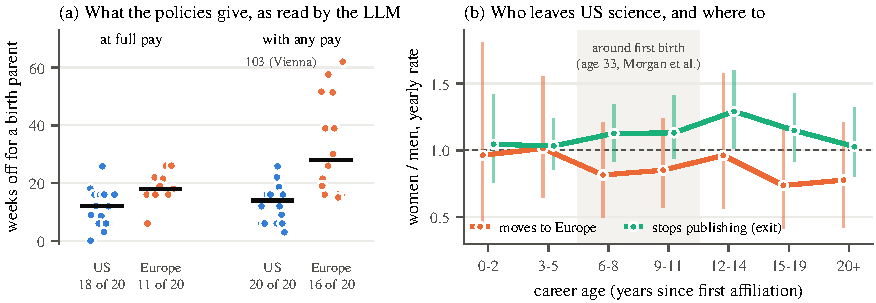
\includegraphics[width=\textwidth]{fig1.pdf}
\caption{(a) Weeks off for a birth parent at 20 US universities and their European twins, extracted by the LLM (bars: medians, ``$n$ of 20'': texts that state it). (b) Women-to-men ratio of yearly rates of leaving US science, with 95\% bootstrap CIs. Shaded: the birth window.}
\end{figure*}

\section{Data}
\textbf{Used in this pilot.} 20 US universities drawn at random from the 80 most productive in OpenAlex \citep{priem2022}, half in states with a state paid family leave program, CU Boulder fixed in, each matched one-to-one to a European \emph{twin} with the closest field mix, size and citations per work (Appendix B). LLM-assisted search on official domains found 92 policy documents, 551,000 words in eight languages. The Wayback Machine I used only to recover blocked pages and to count archived versions. For careers, random samples of OpenAlex authors ever affiliated with a US institution. Career age is years since an author's first affiliation, and since births are not observed, the \emph{birth window} is career ages 6--11, where a first birth at the faculty average age of 33 \citep{morgan2021} falls if careers start in the mid-twenties. \textbf{Added in the full study:} the AARC faculty census used by \citet{spoon2023}, the 2018 collection \citep{morgan2018} as ground truth, the EPLP national leave panel \citep[21 countries, 1970--2024;][]{spitzer2026}, and every archived policy version since 2011. \emph{Permissions:} the policies are public (not redistributed), OpenAlex is CC0, AARC is licensed and needs its holders' agreement, and linking it to OpenAlex needs IRB review. Results are reported in aggregate.

\section{Language features (operationalization)}
The NLP part is a five-step pipeline (Appendix A). \emph{Retrieval}: an LLM agent with web search finds the official pages, a script downloads them. \emph{Passage selection}: contracts of 50,000--80,000 words are cut to 120-word windows that mention leave in any of the eight languages. \emph{Extraction}: an LLM reads the passages for one reference person, a tenure-track assistant professor with two years of service and a first child, and fills a ten-field codebook (Table A1), converting units and quoting the sentence behind every field, which a script checks against the document. \emph{Framing} is gendered (maternity, mother), neutral (parent, birth parent) or mixed. \emph{Versions}: the same extraction on every archived version dates each policy change. The weeks are what a woman choosing between two offers would compare, close to the 10-week measure of \citet{morgan2021}, and the framing is the cultural part: whom the institution expects to do the caring.

\section{Feasibility test}
\textbf{Documents: easy in the US, hard in Europe.} I found official rules for all 20 US universities (the Wayback Machine returned seven of the nine pages that blocked downloads). Four of the 20 European twins have no public page on staff leave, only an intranet behind a login, and for them the public text is national law or a sector agreement.

\textbf{Extracting and checking.} Claude Opus 5.5 coded all 40 universities. GPT-6.1 Terra and Grok 4.7 Fast, as stand-ins for human coders, coded 10 universities blind on six fields. Claude agrees with GPT on 51 and with Grok on 50 of the 60 cells, with at least one of them on 58. The numbers almost always match (all three agree on 9 of 10 birth-parent weeks), the labels less (5 of 10 framings), mostly in cases the codebook does not decide yet.

\textbf{What the policies say.} A birth parent gets a median of 12 weeks at full pay at the US universities and 18 at their twins, higher in Europe in 7 of the 9 pairs where both are stated (Figure~1a). But the European number can be read for only 11 of 20 twins, because most others point to national law without stating it. The framing splits by continent: 17 of 20 US texts are neutral, 18 of 20 European texts gendered or mixed. Yet 9 of the 20 US policies tie the benefit to being the ``primary caregiver'', so neutral words still ask one parent to declare the caring (Appendix A).

\textbf{Careers (H1): no sign of a pull to Europe.} Of the sampled authors, 8,943 began their careers in 1990--2018 and have a first name a dictionary could gender \citep{genderguesser}, 3,651 of them women. In the birth window the women-to-men ratio for moves to Europe is below 1 (0.81 [0.50, 1.21] at career ages 6--8) and for exits slightly above 1 (1.13 [0.92, 1.35]), with no interval excluding 1 (Figure~1b). The only clear gap is in exits at 12--14 (1.29 [1.01, 1.60]), close to the tenure decision. With small counts and names as a weak proxy, this is a reason for the full test. Most moves to Europe are returns: 65\% of the movers began their careers there (Appendix B).

\section{Relation to existing work}
Leave policies exist for 205 US and Canadian universities \citep{morgan2018}, top economics departments \citep{antecol2018} and European countries \citep{spitzer2026}. Career studies measure the cost of parenthood \citep{morgan2021}, attrition \citep{spoon2023}, prestige \citep{wapman2022} and migration, where women are less mobile \citep{zhao2023}, but none links careers to leave policies. LLM coding works on some tasks and not others \citep{bamman2024,than2025}, and uncertain LLM labels can still support valid conclusions \citep{gligoric2025}. I add a panel of policies read from text, on both continents and over time, linked to where people go.

\section{Methods considered, and rejected}
\emph{Hand-coding}: one snapshot of 400 US universities and their European matches is about 11 million words at the pilot's rate. \emph{Keyword search} misses units, caps (``up to''), conditions and references to national law. \emph{One long prompt}: given ten policies in one file, Grok reported four as missing, as in the long-context failures of \citet{karpinska2024}, so the pipeline reads one university at a time. \emph{Inferring births from acknowledgments or publication gaps} is noisy and too private. \emph{Surveys of leavers}, best for reasons \citep{spoon2023}, come later.

\section{Limitations, ethics, next steps}
A policy on paper is not its use (91.8\% of eligible mothers but 62.1\% of fathers took leave, \citealp{morgan2021}). Names are a binary and weak proxy for gender, OpenAlex affiliations are noisy, the birth window overlaps the end of graduate training and the tenure decision, and the 2025 US funding cuts confound the latest years, so the main estimates stop before 2025. The pilot shows associations only. \textbf{Next} (Appendix C): all PhD-granting US universities and their European matches yearly from 2011, human coders, the destination of everyone who leaves AARC, H1--H3 in a competing-risks model with a staggered difference-in-differences from the state programs (California 2004 to Colorado 2024), and the cost of the exits a one-semester floor would prevent, for a brief to universities and legislators.

\section*{Team}
Antoni Czolgowski (solo): question, design, data, experiments and writing.

\section*{Acknowledgments}
Readings that shaped the idea: \citet{gligoric2025}, \citet{bamman2024}, \citet{than2025} and \citet{karpinska2024}, which I presented in class as the archaeologist. AI use: Claude Opus 5.5 (in Claude, medium reasoning) helped me find the official policy pages, write the twin matching, collection and OpenAlex code, run the codebook extraction, make the figure and edit the text. GPT-6.1 Terra (ChatGPT, medium reasoning) and Grok 4.7 Fast were the second and third coders, run by me in fresh chats with the same rules. Code, codebook and extracted fields: \url{github.com/AntoniCzolgowski/parental-leave-nlp4ca}.

\small
\begin{thebibliography}{99}
\bibitem[Antecol et~al.(2018)]{antecol2018} H. Antecol, K. Bedard, J. Stearns. 2018. Equal but inequitable: Who benefits from gender-neutral tenure clock stopping policies? \emph{American Economic Review} 108(9):2420--2441.
\bibitem[Bamman et~al.(2024)]{bamman2024} D. Bamman, K. K. Chang, L. Lucy, N. Zhou. 2024. On classification with large language models in cultural analytics. \emph{Computational Humanities Research (CHR) 2024}, CEUR 3834.
\bibitem[Gligori\'c et~al.(2025)]{gligoric2025} K. Gligori\'c, T. Zrnic, C. Lee, E. Cand\`es, D. Jurafsky. 2025. Can unconfident LLM annotations be used for confident conclusions? \emph{NAACL 2025}.
\bibitem[gender-guesser(2016)]{genderguesser} gender-guesser. 2016. Python package, based on J. Michael's name dictionary. \url{pypi.org/project/gender-guesser}.
\bibitem[Karpinska et~al.(2024)]{karpinska2024} M. Karpinska, K. Thai, K. Lo, T. Goyal, M. Iyyer. 2024. One thousand and one pairs: A ``novel'' challenge for long-context language models. \emph{EMNLP 2024}.
\bibitem[Morgan et~al.(2018)]{morgan2018} A. C. Morgan, S. F. Way, M. Galesic, D. B. Larremore, A. Clauset. 2018. Paid parental leave at US and Canadian universities. Online dataset, CU Boulder and Santa Fe Institute.
\bibitem[Morgan et~al.(2021)]{morgan2021} A. C. Morgan, S. F. Way, M. J. D. Hoefer, D. B. Larremore, M. Galesic, A. Clauset. 2021. The unequal impact of parenthood in academia. \emph{Science Advances} 7(9):eabd1996.
\bibitem[Priem et~al.(2022)]{priem2022} J. Priem, H. Piwowar, R. Orr. 2022. OpenAlex: A fully-open index of scholarly works, authors, venues, institutions, and concepts. arXiv:2205.01833.
\bibitem[Spitzer et~al.(2026)]{spitzer2026} S. Spitzer, A. Lemoine, Z. Song, et al. 2026. The European Parenting Leave Policies (EPLP) dataset: Leave duration entitlements for 21 countries from 1970 to 2024. \emph{Demographic Research} 54(31):987--1008.
\bibitem[Spoon et~al.(2023)]{spoon2023} K. Spoon, N. LaBerge, K. H. Wapman, et al. 2023. Gender and retention patterns among U.S. faculty. \emph{Science Advances} 9(42):eadi2205.
\bibitem[Than et~al.(2025)]{than2025} N. Than, L. Fan, T. Law, L. K. Nelson, L. McCall. 2025. Updating ``the future of coding'': Qualitative coding with generative large language models. \emph{Sociological Methods \& Research} 54(3):849--888.
\bibitem[Wapman et~al.(2022)]{wapman2022} K. H. Wapman, S. Zhang, A. Clauset, D. B. Larremore. 2022. Quantifying hierarchy and dynamics in US faculty hiring and retention. \emph{Nature} 610:120--127.
\bibitem[Zhao et~al.(2023)]{zhao2023} X. Zhao, A. Akbaritabar, R. Kashyap, E. Zagheni. 2023. A gender perspective on the global migration of scholars. \emph{PNAS} 120(10):e2214664120.
\end{thebibliography}
\onecolumn
\normalsize
\setlength{\parskip}{4pt}
\section*{Appendix A. The NLP pipeline in detail}
\textbf{Retrieval.} For each university an LLM agent (Claude, with web search) looked for the official page or PDF with the current faculty parental leave rules, restricted to the university's and the government's domains, and had to confirm that the page states the rules. A script then downloaded every page and converted HTML, PDF and Word files to text. Nine US pages refused automated download (HTTP 403 or a certificate error), and the Wayback Machine's latest copy recovered seven. For Europe the agent also collected the national government page on maternity and parental leave, because university pages often only refer to it. Four twins (Montpellier, Florence, Aix-Marseille, Copenhagen) have no public staff leave page, and Delft, Amsterdam, LMU, Bonn, Gothenburg and Liverpool publish only summaries, with the full rules on intranets. In total 92 documents, 551,000 words: 36 US documents (292,000 words) and 56 European ones (260,000 words), in English, German, French, Italian, Spanish, Dutch, Swedish and Danish. For six US policy pages the Wayback Machine holds between 3 and 70 captures since 2012, and the University of California's policy PDF alone has 9 versions with different content since 2014. Page hashes overcount changes (the NYU handbook page has 31 hashes in 33 captures), so versions are compared on the extracted fields, which I have not run yet.

\textbf{Passage selection.} Short documents (under 2,500 words) are kept whole. Longer ones (union contracts at Cincinnati and Florida State, the Case Western handbook, the Dutch universities' collective agreement) are cut into 120-word windows. A window is kept if it matches a list of leave terms in the eight languages (parental, maternity, paternity, childbirth, adoption, bonding, caregiver, tenure clock, modified duties, FAMLI, PFML, Mutterschutz, Elternzeit, Elterngeld, Karenz, congé maternité, congedo, föräldraledighet, barsel, zwangerschapsverlof, ouderschapsverlof, permiso por nacimiento, and others), together with its two neighbors. A first version kept whole paragraphs and lost the leave sections of the Duke and Case Western handbooks, whose text came as one long paragraph. The window version fixed it.

\textbf{Extraction.} The LLM reads each university's passages separately (one long prompt with many universities fails, see Section 6) and fills the codebook in Table A1 for the reference person. It converts units (a semester is 16 weeks, a quarter 11, a month 4.3, 40 hours one week, five working days one week), counts statutory pay together with university pay only when the text states both, and does not add facts from its own knowledge. For every field it gives a verbatim quote of at most 25 words and a confidence (high, medium, low). A script checks that every quote appears in the document. The extraction itself caught two data errors: the Wayback copies of Michigan's pages had been saved compressed and read as garbage, and the Duke and Case Western sections were cut off.

\begin{center}\small
\begin{tabular}{@{}p{3.6cm}p{6.2cm}p{6.4cm}@{}}
\toprule
Field & Definition & Example evidence quote (extracted value) \\ \midrule
Birth parent, full-pay weeks & weeks released from all duties at 90--100\% pay & CU Boulder: ``Tenured and Tenure Track Faculty receive 18 weeks of parental leave at full pay'' (18) \\
Birth parent, any-pay weeks & weeks with any pay, statutory included & Nottingham: ``26 weeks' leave on full pay* (inclusive of any SMP)'' (26 at full, 39 any) \\
Non-birth parent, full-pay weeks & as above, for the partner & Zurich: ``Der bezahlte Urlaub beträgt zwei Wochen.'' (2) \\
Teaching relief & semesters without teaching, at full pay, on top of the leave & NYU: one semester of workload relief at full salary (1) \\
Tenure clock & automatic, on request, none, not applicable & Michigan: ``a woman who bears one or more children during her tenure probationary period shall, upon written request\ldots'' (on request) \\
Primary-caregiver clause & a benefit depends on being the primary caregiver & CMU: ``and who is the primary care giver of the child, is entitled to a one semester paid leave of absence'' (yes) \\
Who pays & university, state or insurance, mixed & Karolinska: university top-up on the state parental benefit (state) \\
Service needed & months of service to qualify & Reading: ``continuously employed with the University for at least 26 weeks'' (6) \\
Relies on outside rules & the text refers to rules it does not state & LMU: Mutterschutz named only by the law's title (yes) \\
Framing & gendered, neutral or mixed & Michigan: ``paid maternity (childbirth) leave and paid parental leave'' (mixed) \\ \bottomrule
\end{tabular}

\smallskip
Table A1. The codebook, with real evidence quotes from the extraction.
\end{center}

\textbf{Results by continent.} Table A2 gives every field for the 20 US universities and their 20 twins. The pattern beyond the weeks: US policies use neutral words (17 of 20), but 9 of 20 tie the benefit to being the primary caregiver, against 5 of 20 in Europe, where the clause mostly comes from the German parental allowance that two parents share. US universities pay the leave themselves (17 of 20), give teaching relief (9 of 19 at least half a semester) and extend the tenure clock (all 18 that mention it), while European rules are mostly paid by the state or social insurance and 11 of 20 twins have no tenure track at all. The non-birth parent gets a median of 6 weeks at full pay in the US (19 texts state it) and 2 in Europe (only 7 do). The caregiver clause is the second least certain field after framing (coders agreed on 7 of 10 universities), and in Europe 15 of 20 texts rely on rules they do not state.

\begin{center}\small
\begin{tabular}{@{}lcc@{}}
\toprule
 & US (20) & European twins (20) \\ \midrule
Birth parent, full-pay weeks: median (texts that state it) & 12 (18) & 18 (11) \\
Birth parent, any-pay weeks: median (texts) & 14 (20) & 28 (16) \\
Non-birth parent, full-pay weeks: median (texts) & 6 (19) & 2 (7) \\
Teaching relief of at least half a semester & 9 of 19 & 1 of 20 \\
Tenure clock: automatic / on request / not applicable / not stated & 6 / 12 / 0 / 2 & 4 / 4 / 11 / 1 \\
Primary-caregiver clause & 9 & 5 \\
Framing: neutral / mixed / gendered & 17 / 3 / 0 & 2 / 10 / 8 \\
Paid by: university / state or insurance / mixed / not stated & 17 / 1 / 2 / 0 & 7 / 8 / 2 / 3 \\
Relies on rules it does not state & 6 & 15 \\ \bottomrule
\end{tabular}

\smallskip
Table A2. Extracted fields by continent (Claude Opus 5.5).
\end{center}

\begin{center}
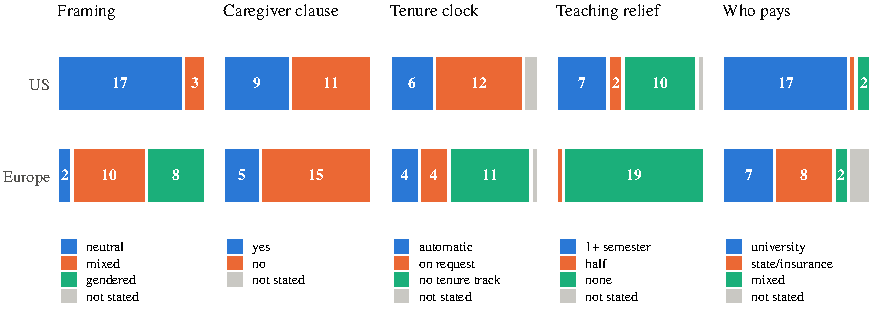
\includegraphics[width=\textwidth]{figA1.pdf}

\smallskip
{\small Figure A1. The categorical fields for the 20 US universities and their 20 European twins (counts). ``Caregiver clause'': a benefit depends on being the primary caregiver.}
\end{center}

\textbf{Agreement with the other coders.} GPT-6.1 Terra and Grok 4.7 Fast coded ten universities (CU Boulder, Princeton, Carnegie Mellon, Michigan, Arizona State, UCL, Reading, Liverpool, Karolinska, Zurich) on six fields, from the same passages, with the rules written as instructions for a human coder (the prompt is in the repository). Numbers count as agreeing within one week.

\begin{center}\small
\begin{tabular}{@{}lcccc@{}}
\toprule
Field (10 universities) & Claude--GPT & Claude--Grok & GPT--Grok & All three \\ \midrule
Birth parent, full-pay weeks & 10 & 9 & 9 & 9 \\
Non-birth parent, full-pay weeks & 10 & 6 & 6 & 6 \\
Teaching relief & 8 & 8 & 8 & 7 \\
Tenure clock & 9 & 9 & 10 & 9 \\
Framing & 7 & 8 & 5 & 5 \\
Primary-caregiver clause & 7 & 10 & 7 & 7 \\ \midrule
Total (60 cells) & 51 & 50 & 45 & 43 \\ \bottomrule
\end{tabular}

\smallskip
Table A3. Agreement between the three coders.
\end{center}

Most disagreements come from three cases the codebook does not decide yet. When the text says nothing about the non-birth parent, Grok wrote 0 weeks and the others left it empty. Mixed and gendered framing overlap for UK policies that say ``maternity'' and ``partner''. And the UK rule that a mother must end her maternity leave before her partner can share it counts as a primary-caregiver clause for GPT but not for Claude or Grok. I will settle these in the codebook before the full run. Agreement between models is not accuracy, because models can share mistakes, which is why the full study adds human coders (Appendix C).

\section*{Appendix B. Twins, samples and definitions}
\textbf{Twins.} For the 200 most productive US and 600 most productive European educational institutions in OpenAlex (17 countries, research institutes and medical schools excluded), each university is described by its share of output across 26 research fields (from its top topics), the log of its number of works and the log of its citations per work. The distance between two universities is the cosine distance of the field shares plus half the absolute difference of each log measure. The 20 US universities were drawn with a fixed seed: 10 from the 80 most productive in states with a state paid family leave program (California, Colorado, Connecticut, Massachusetts, New Jersey, New York, Oregon, Rhode Island, Washington, DC), CU Boulder among them, and 10 from the other states. Twins come from an optimal one-to-one assignment with at most four per country. Michigan has no European university of its size, so its pair is weak.

\begin{center}\small
\begin{tabular}{@{}llcllc@{}}
\toprule
US university & State & Paid leave program & European twin & Country & Distance \\ \midrule
CU Boulder & CO & yes & University of Liverpool & UK & 0.22 \\
UCLA & CA & yes & University College London & UK & 0.14 \\
New York University & NY & yes & LMU Munich & DE & 0.31 \\
Princeton & NJ & yes & University of Zurich & CH & 0.17 \\
Oregon State & OR & yes & University of Reading & UK & 0.27 \\
Washington State & WA & yes & Université de Montpellier & FR & 0.42 \\
Tufts & MA & yes & University of Basel & CH & 0.23 \\
UC San Diego & CA & yes & Karolinska Institutet & SE & 0.82 \\
University of Rochester & NY & yes & University of Bonn & DE & 0.03 \\
University at Buffalo & NY & yes & University of Florence & IT & 0.12 \\
University of Kentucky & KY & no & University of Nottingham & UK & 0.27 \\
Georgia Tech & GA & no & TU Delft & NL & 0.34 \\
University of Cincinnati & OH & no & University of Naples Federico II & IT & 0.19 \\
Florida State & FL & no & Universidad Autónoma de Madrid & ES & 0.09 \\
Case Western Reserve & OH & no & University of Gothenburg & SE & 0.22 \\
Carnegie Mellon & PA & no & University of Amsterdam & NL & 0.66 \\
Arizona State & AZ & no & Aix-Marseille Université & FR & 0.15 \\
Duke & NC & no & KU Leuven & BE & 0.27 \\
University of Michigan & MI & no & University of Copenhagen & DK & 1.13 \\
Louisiana State & LA & no & University of Vienna & AT & 0.19 \\ \bottomrule
\end{tabular}

\smallskip
Table B1. The 20 pairs.
\end{center}

\textbf{Careers.} Three random samples of 10,000 OpenAlex authors ever affiliated with a US institution and with 10 to 1,000 works (29,915 distinct authors), and one sample of 10,000 authors ever in the US whose last known institution is in Europe (the movers sample). For each author I take the yearly affiliation countries. An author is at risk in every US year up to the last one, if they have at least two US years. A \emph{move to Europe} is a last US year followed by at least two years at an institution in one of 17 European countries (most of the EU plus the UK, Switzerland and Norway), a \emph{move elsewhere} the same for other countries, and an \emph{exit} a last US year in 2020 or earlier with no affiliation after it. Gender comes from the first name with the gender-guesser dictionary, keeping only ``female'' and ``male'' (37.5\% of names are not gendered, and the dictionary fails more often on non-European names, which biases the sample). The analytic sample is 8,943 authors (3,651 women, 5,292 men) whose careers began in 1990--2018, with 55,357 person-years in the US in 2000--2020, and 201 moves to Europe by women and 380 by men. The rate ratio is the women's yearly rate divided by the men's, by career-age group, with 95\% intervals from 300 bootstrap resamples of authors. In the movers sample, 1,699 authors meet the definition of a move to Europe with a career that began in 1990--2018 and a gendered name, and 65\% of them had their first affiliation in Europe.

\section*{Appendix C. The full study}
\textbf{(1) Policies.} Collect the rules of every PhD-granting US university in AARC and of its closest European match (without the one-to-one rule and the cap), every year since 2011, with the archived versions from the Wayback Machine, and join the European rules to the national layer from EPLP. At the pilot's rate this is about 11 million words per yearly snapshot, so the extraction runs on an open model on CU's Alpine cluster as well as on Claude, and the two are compared.

\textbf{(2) Validation.} Check the extracted weeks against the 2018 collection of 205 universities, and double-code a random 10\% of policy versions with trained student coders or Prolific workers screened with a short quiz on the codebook. A panel of LLM coders from different companies codes everything, and only the documents where they disagree go to humans. The remaining error is carried into the regressions with the method of \citet{gligoric2025}.

\textbf{(3) Destinations.} Link every person who leaves a faculty job in AARC to OpenAlex and record their next affiliation: another US university, a European university, another country, or none.

\textbf{(4) Model.} For each faculty member $i$ in year $t$, a competing-risks (multinomial logit) model of five outcomes $k$: stay, move within the US, move to Europe, move elsewhere, exit,
\[ \log \frac{P(y_{it}=k)}{P(y_{it}=\text{stay})} = \alpha_k + \beta_k W_i + \gamma_k B_{it} + \delta_k W_i B_{it} + \theta_k W_i B_{it} P_{jt} + \lambda_k W_i B_{it} F_{jt} + X_{it}\eta_k , \]
where $W_i$ is a woman, $B_{it}$ the birth window, $P_{jt}$ at least a semester of paid leave at university $j$ in year $t$, $F_{jt}$ the framing, and $X_{it}$ field, the prestige of the US institution \citep{wapman2022}, rank, PhD country and year. H1 is about $\delta_k$ for Europe against exit, H2 about $\theta_k$, H3 about $\lambda_k$. Returns home are separated by the country of the first affiliation. For a causal estimate, the state programs started in different years (California 2004, New Jersey 2009, Rhode Island 2014, New York 2018, Washington 2020, Massachusetts 2021, Connecticut 2022, Oregon 2023, Colorado 2024), and the Wayback Machine dates the changes in university policies, so $\theta$ can be estimated as a staggered difference-in-differences, women against men, before against after, adopters against not yet adopters.

\textbf{(5) Calculations.} From the fitted model, the number of women's exits a one-semester floor would have prevented each year, and their cost to a university: a new faculty search, a new start-up package, and the research output the person would have produced, using publication rates before the exit.

\textbf{(6) Brief.} A short brief for university leaders and state legislators, with the policy comparison per state and the estimated cost of doing nothing.

\end{document}
